\chapter{Example Workflows}
\index{Workflows}

\section{Creating a Hydrogeological Subsurface Mesh}
\label{sec:dataexplorer:workflow}

\begin{figure}[!h]
\begin{center}
\subfloat[Surface model data]{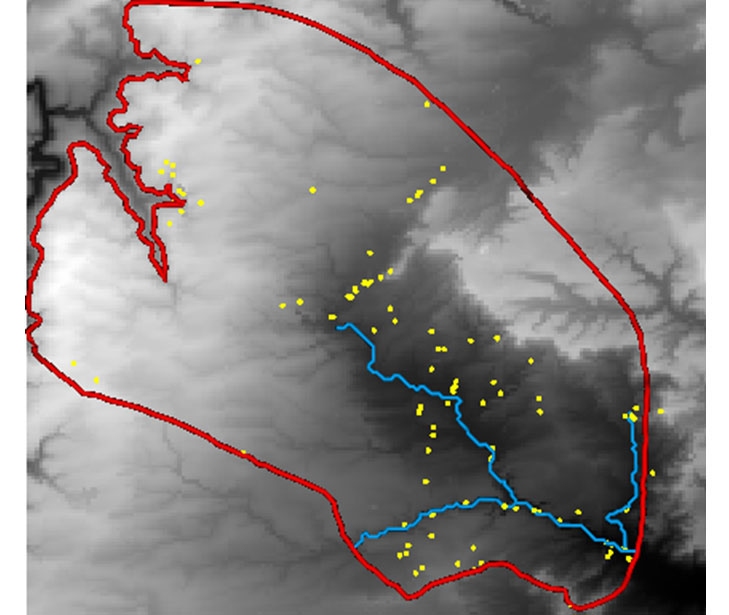
\includegraphics[width=0.48\linewidth]{ammer_gis.png}\label{fig:kr:ammer_gis}}\enspace
\subfloat[Surface model data]{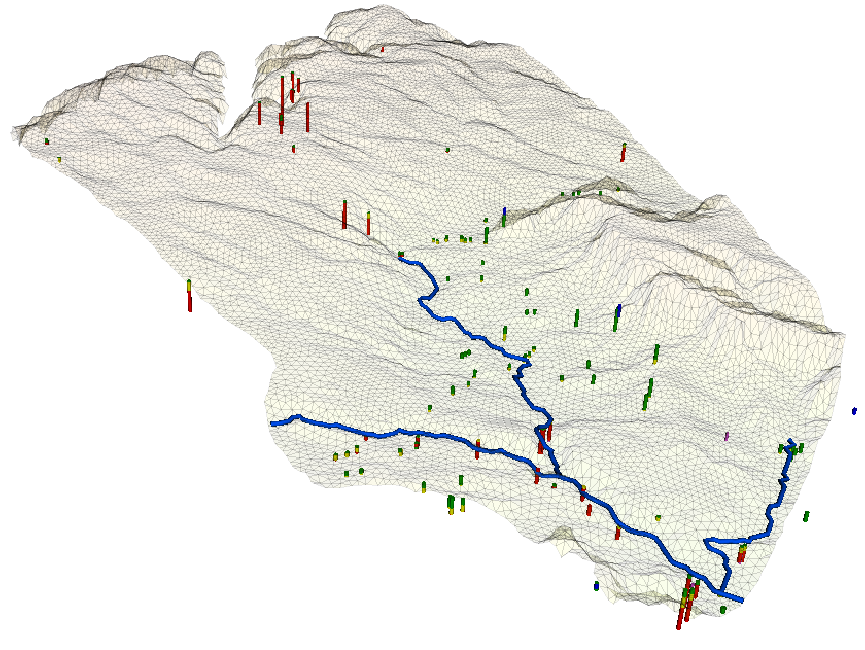
\includegraphics[width=0.48\linewidth]{ammer_sfc.png}\label{fig:kr:ammer_2d}}\\
\subfloat[Subsurface model]{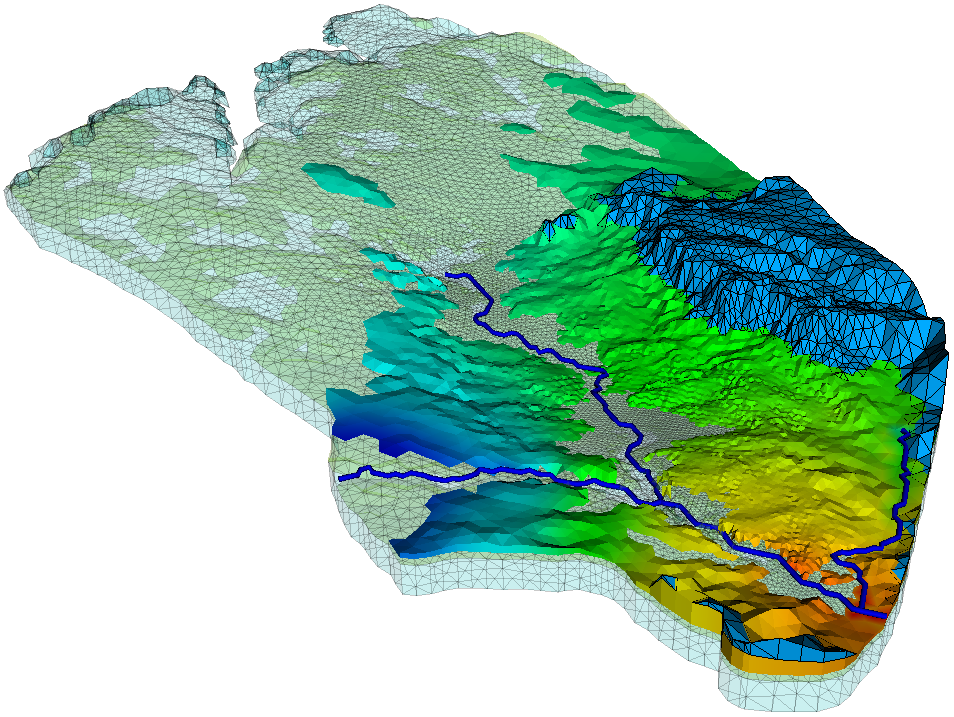
\includegraphics[width=0.48\linewidth]{ammer_3d.png}\label{fig:kr:ammer_3d}}\enspace
\subfloat[Simulation results]{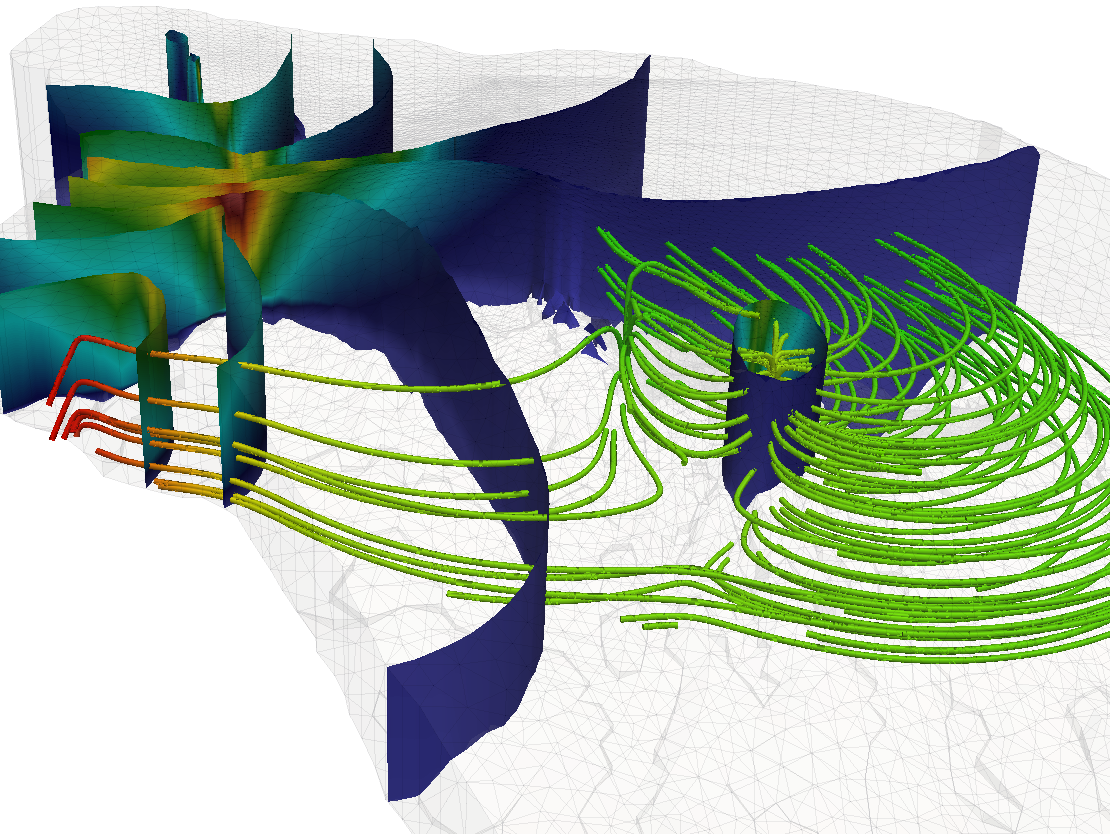
\includegraphics[width=0.48\linewidth]{ammer_sim.png}\label{fig:kr:ammer_sim}}
\end{center}
\caption{Visualization of data sets at various stages of the modeling process. (a) Input data from geographic information systems (GIS). (b) 3D surface model based on GIS data. (c) Subsurface model with layers interpolated based on borehole data. Different information is displayed for each geological layer. (d) Representation of simulation results using established visualization techniques such as isosurface and streamtracers.}
\label{fig:kr:vis}
\end{figure}

\subsection{Input Data}

As processes are simulated using the finite element method, adequate domain discretizations -- i.e. meshes -- need to be created either using the \emph{OpenGeoSys Data Explorer} or by employing other software.

For generating such a mesh using the \emph{Data Explorer}, geometric input data needs to be imported into the framework to define basic requirements such as the boundary of model region. This is done by selecting \cmd{File \ra Import files...} from the main menu and then selecting the appropriate file type. If external software has been employed, the corresponding mesh for the model region needs to be imported in a similar manner. The \emph{Data Explorer} supports a large number of established geo-scientific data formats, see figure \ref{fig:interfaces} for an overview. After selecting a specific file type, a file-open-dialogue will pop up and after choosing a file it is imported into the program.

If imported data will be needed again within \emph{OpenGeoSys} in the foreseeable future or if data has been somehow modified using the \emph{Data Explorer}, the respective data set should be saved to a native \emph{OpenGeoSys} file. To do this, the \emph{Data View} tab where the data set is listed (i.e. Geometry, Meshes, Stations or Modelling) needs to be selected and upon clicking the little disk-symbol on top of the tab the data will be saved. Geometric data will be written into a gml-file, meshes to vtu-files, station-data in stn-files and modelling data (i.e. Boundary conditions) in cnd-files. This process is repeated for every data set that needs to be converted and saved to an \emph{OpenGeoSys} format.

\begin{figure}[t]
\begin{center}
\subfloat[Feature embedding]{\frame{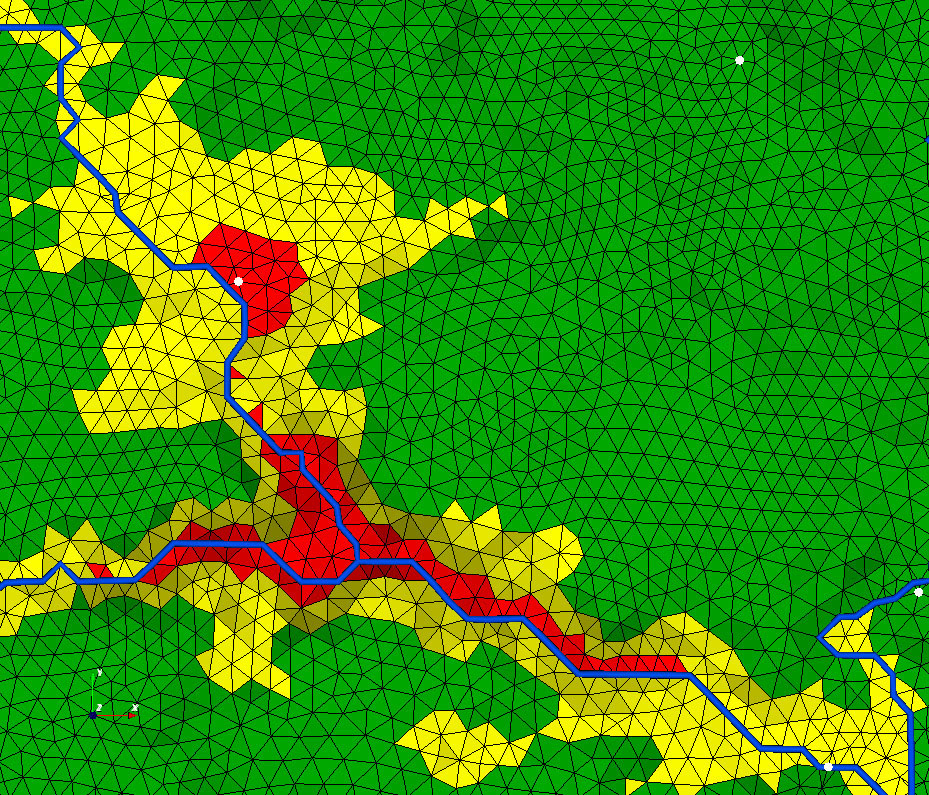
\includegraphics[width=.33\linewidth]{triangulation.png}}\label{fig:kr:triangulation}}\enspace
\subfloat[Mesh quality]{\frame{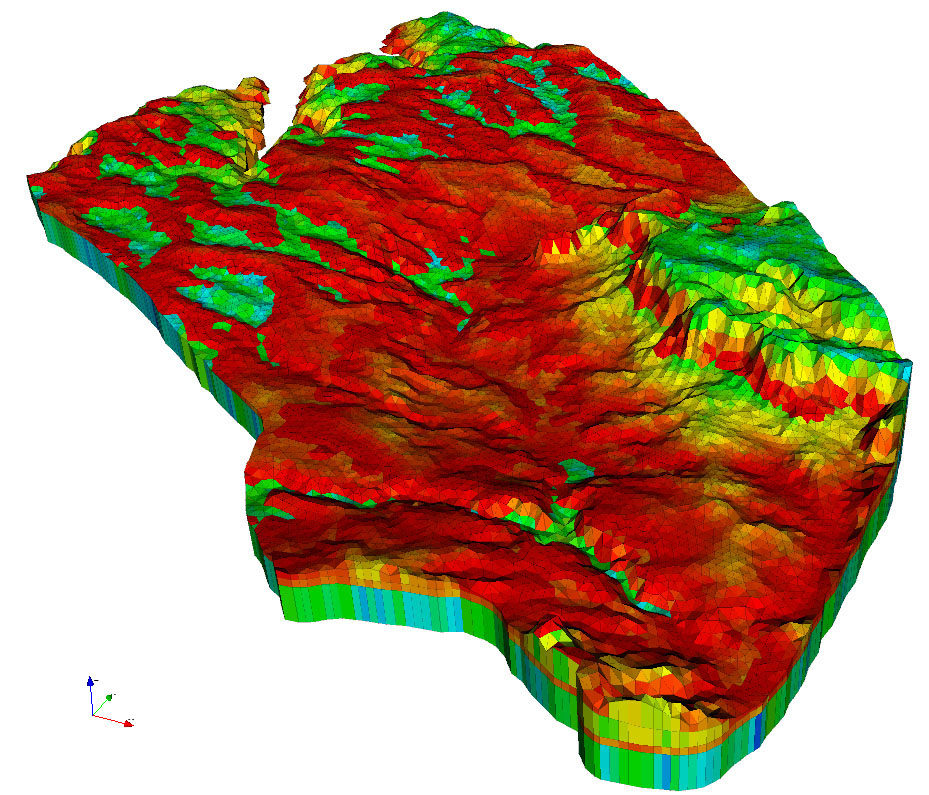
\includegraphics[width=.33\linewidth]{qual_edge_ratio.png}}\label{fig:kr:edgeratio}}\enspace
\subfloat[Element selection]{\frame{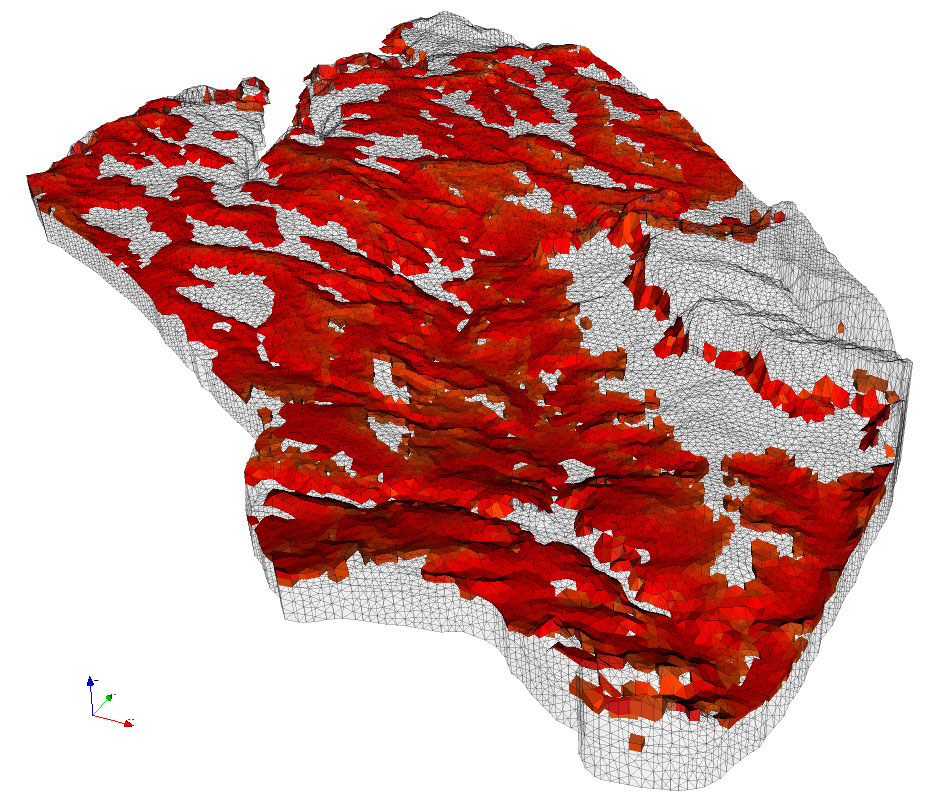
\includegraphics[width=.33\linewidth]{qual_edge_ratio_thresh.png}}\label{fig:kr:selection}}
\end{center}
\caption{Mesh quality validation: (a) Embedding geometric information representing rivers (blue) and wells (white) into the mesh structure. (b) Element quality based on edge ratio. Red/orange signifies large differences in edge length, green/blue signifies roughly equilateral elements. (c) Further analysis reveals that elements with a large edge ratio are the result of a thin surface layer.}
\label{fig:kr:meshqual}
\end{figure}

\subsection{Creating a 2D Surface Mesh}

The minimum requirements for creating a 2D mesh is a polygon representing the outer boundary of the model region as well as a digital elevation model (DEM) to derive the elevation at any point within the region (Fig.~\ref{fig:kr:ammer_gis}). Typically such data can be prepared using geographic information systems such as \emph{ArcGIS} but any supported data format will do.

In a first step, a triangulation of the area bounded by the polygon will be created. For detailed simulations, it is preferable to integrate additional data into the mesh that will be relevant for the model later on. Examples for this case study include the courses of rivers as well as a number of boreholes and wells. Boundary conditions will later be applied to these objects and integrating them into the mesh at the beginning of the model setup will ensure a less error-prone configuration of the model later on. See figure~\ref{fig:workflow:2Dmesh} for the effect of integrating these geometric objects when generating the mesh.
The process is started by selecting \cmd{Tools \ra Mesh Generation...} from the main menu. A dialog will open, where all data sets that have been loaded and might potentially be included into the new mesh are listed on the left hand side. By selecting data sets and moving them to the right hand side of the dialog they are added as constraints to be eventually included into the new mesh. When clicking on the \cmd{Advanced}-tab, a number of parameters for creating the mesh may be adjusted. Most importantly, the user can decide if the resulting mesh should have a homogeneous element size (all elements have roughly the same size as much as this is possible given the input data) or if the mesh should be adaptively refined towards geometrical features. This dialog also allows to change some weights employed by the meshing algorithm, with the general gist that smaller numbers will result in a finer mesh. 

When clicking \cmd{OK}, the 2D FEM mesh generator \emph{GMSH}~\cite{geuzaine:gmsh} is employed for creating
a 2D triangulation with elevation $z=0$ for all mesh nodes.

For a more detailed explanation on generating meshes from geometry, see section \ref{meshcreation}.

\begin{figure}[!h]
\begin{center}
\subfloat[Boundary only]{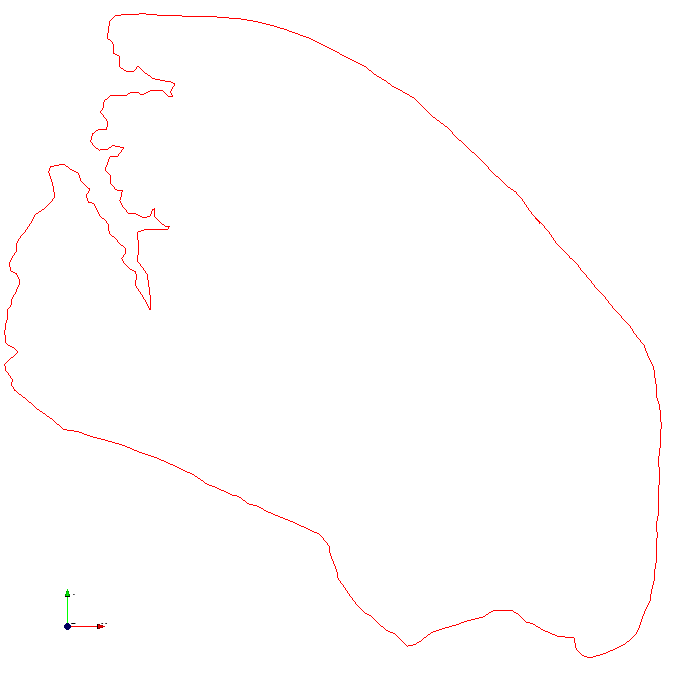
\includegraphics[width=0.3\linewidth]{ammer_geo1}}\enspace
\subfloat[With streams added]{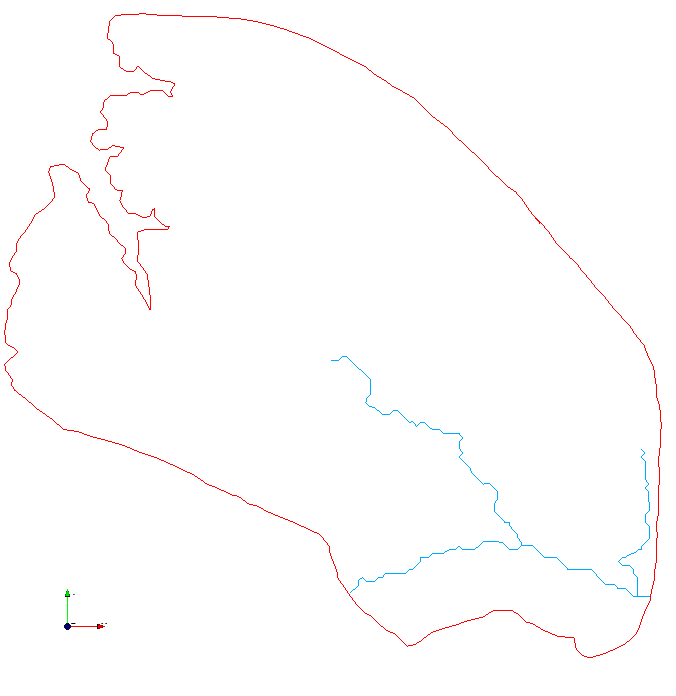
\includegraphics[width=0.3\linewidth]{ammer_geo2}}\enspace
\subfloat[With boreholes added]{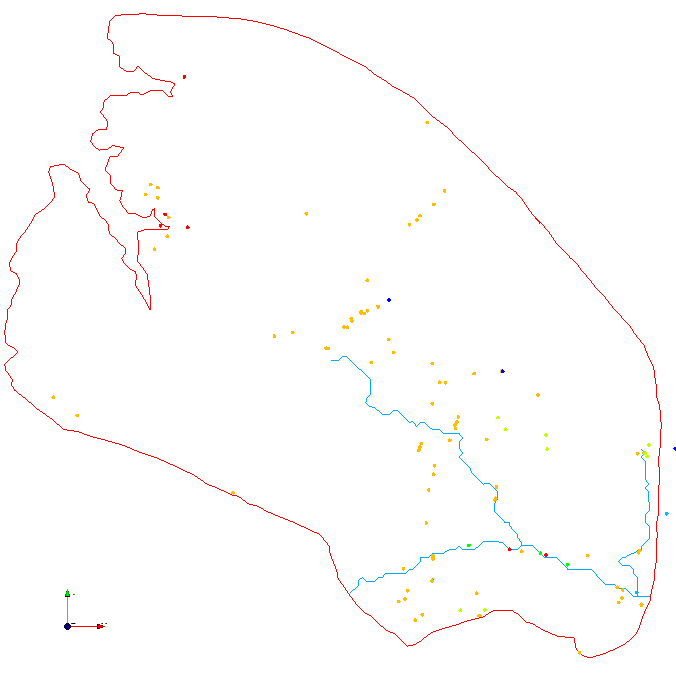
\includegraphics[width=0.3\linewidth]{ammer_geo3}}\\
\subfloat[Mesh from boundary]{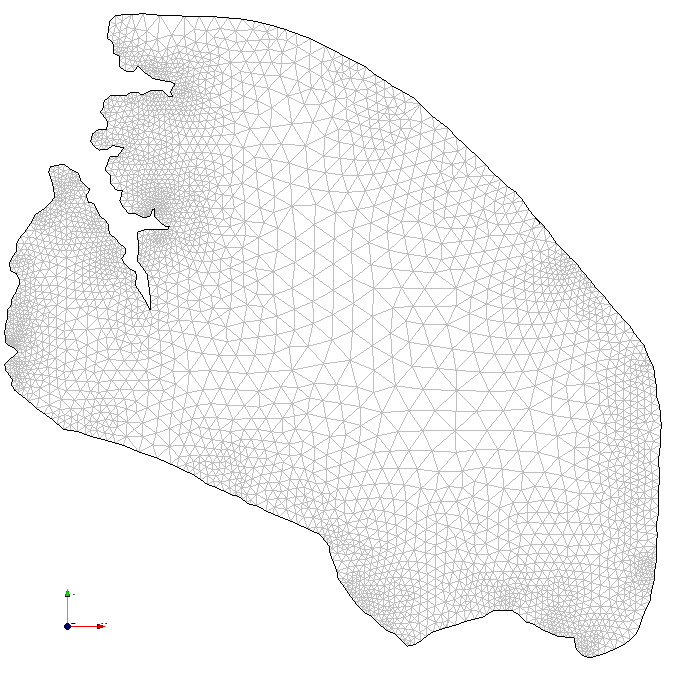
\includegraphics[width=0.3\linewidth]{ammer_mesh1}}\enspace
\subfloat[Including streams]{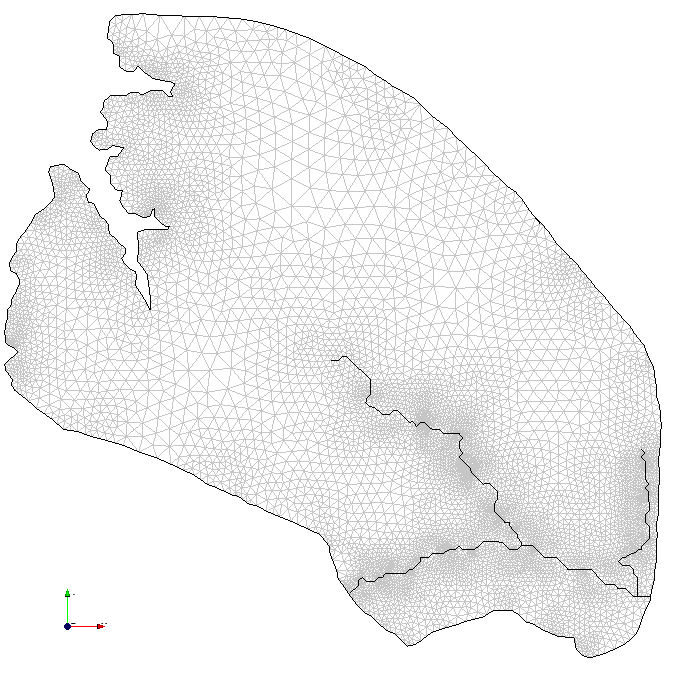
\includegraphics[width=0.3\linewidth]{ammer_mesh2}\label{fig:ammer-mesh2}}\enspace
\subfloat[Including streams and boreholes]{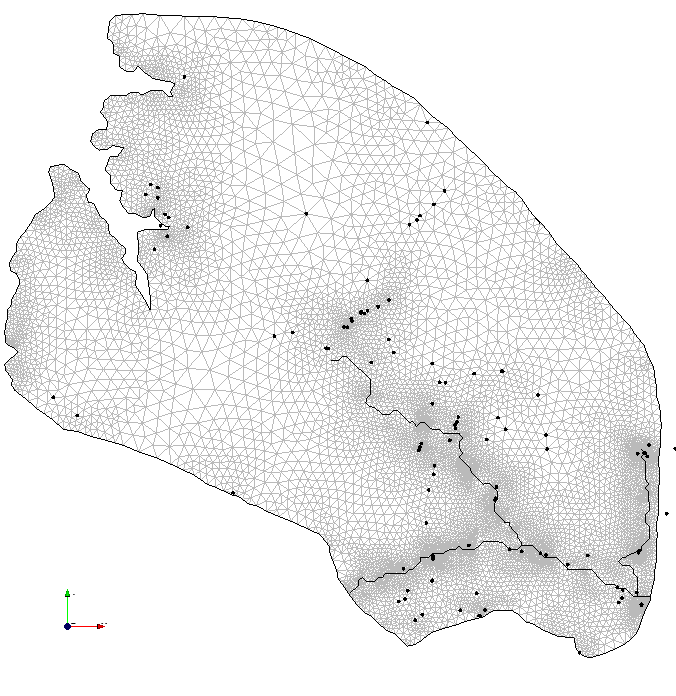
\includegraphics[width=0.3\linewidth]{ammer_mesh3}\label{fig:ammer-mesh3}}\\
\subfloat[Mesh from boundary]{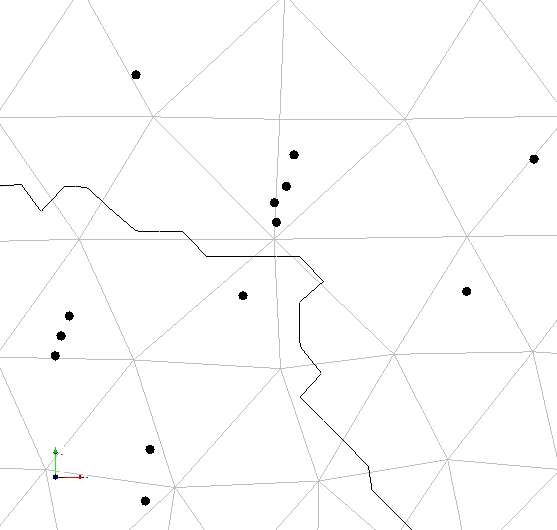
\includegraphics[width=0.3\linewidth]{ammer_meshgeo1}}\enspace
\subfloat[Including streams]{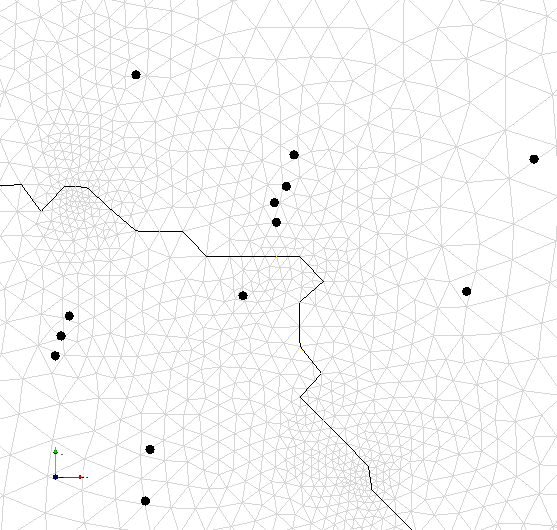
\includegraphics[width=0.3\linewidth]{ammer_meshgeo2}}\enspace
\subfloat[Including streams and boreholes]{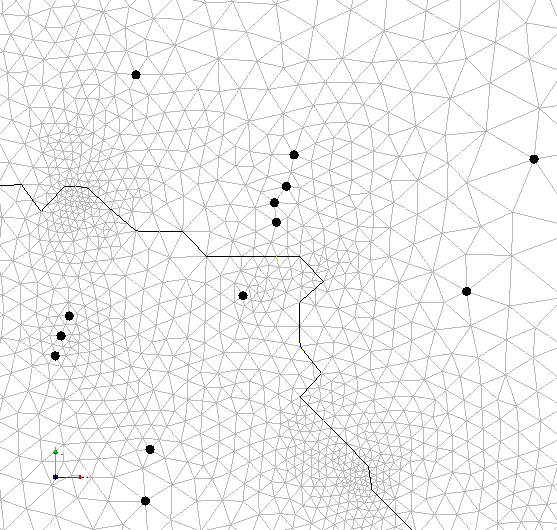
\includegraphics[width=0.3\linewidth]{ammer_meshgeo3}}\\
\end{center}
\caption{Effect of adding information to the meshing process. The upper row shows geometric input data, with one data set added in each column. The resulting meshes are depicted in the second row. The meshes in figures~\ref{fig:ammer-mesh2} and \ref{fig:ammer-mesh3} have a similar refinement but in one mesh boreholes are located directly on mesh nodes and in the other mesh they are not. The bottom row gives a close-up of this effect to visualise how geometric information matches mesh nodes and edges if it has been integrated into the meshing process.\label{fig:workflow:2Dmesh}}
\end{figure}

In a second step, this coplanar mesh will be adjusted into an actual representation of the surface of the domain. This is done by mapping the elevation of mesh nodes based on an interpolation of the DEM of the region.  This can be done by right-clicking on the newly created 2D-mesh in the Mesh Data View and selecting \cmd{Edit mesh...}. When asked for the number of (subsurface) mesh layers, the input should be kept at $0$ since no subsurface layers need to be added at this stage. The dialog will then ask for the location of the DEM used for mapping and upon clicking \cmd{OK} the node elevations will be adjusted (Fig.~\ref{fig:kr:ammer_2d}). The DEM should cover the entire area enclosed by the polygon. For parts of the model area where no DEM information is available, a default value will be used. A triangulated representation of the surface area in the model region is created as a result and a visualization of this data set in 3D space is shown in the framework's render window. Further etails on that topic are given in section \ref{meshondemmapping}.


\subsection{Creating and Mapping Subsurface Layers}

Given the 2D mesh created in the last step, it is now possible to extrude this mesh into a 3D subsurface representation. Note that this surface need not necessarily be mapped based on DEM before creating a 3D mesh. However, performing the mapping step allows for a preliminary analysis of the surface and as such is a useful step for avoiding errors when applying other surface-related algorithms later on.

The 2D mesh should be right-clicked and \cmd{Edit mesh...} needs to be selected again. This time the number of desired subsurface layers needs to be entered before pressing \cmd{Next}.

There are two options for adding new layers to a 2D meshes:
\begin{enumerate}
\item Layers may have a constant thickness (although the thickness of different layers may vary)
\item Layer thickness may be based on elevation maps of subsurface layer boundaries in raster format (i.e. DEMs of layer boundaries, usually interpolated from borehole data)
\end{enumerate}

Depending on which option has been chosen, either the thickness of each layer has to be specified or, alternatively, the path to a DEM raster for each layer boundary needs to be selected.
In addition to layer boundaries, a DEM (i.e. Surface elevation) may be specified again, optionally. If a DEM is given, it will be used for cutting all information from interpolated layers that is located above the surface level specified in this file. This step might be necessary when using interpolated subsurface boundaries, to avoid the domain extending above the actual surface.

The dialog also allows to specify the type of domain discretization by offering the choice between creating prism or tetrahedra elements. Note that for the second option no actual 3D mesh is created. Instead, a 3D geometry for use in the open-source 3D FEM mesh generator \emph{TetGen}~\cite{tetgen:software} will be displayed as well as written into file. The result is a 3D mesh where each element has an ID indicating which material group (or layer) it belongs to (Fig.~\ref{fig:kr:ammer_3d}). Using the 3D visualisation of the \emph{Data Explorer} these different material groups will be displayed using different colors.

Note that subsurface layers can only be added to 2D meshes. Once layers have been added, the dimension of the mesh changes to 3D and adding additional layers automatically is no longer possible using the \emph{Data Explorer}.

Details on adding layers of fixed thickness can be found in section \ref{fixedsizelayers}, information for adding layers based on subsurface DEMs can be found in section \ref{meshondemmapping}.

\subsection{Quality Assurance}

Creating domain discretizations from complex input data might result in meshes containing suboptimal or even degenerated elements. While a lot of common sources of errors are automatically detected and, if possible, avoided, multiple complex datasets might still potentially result in a set of non-trivial geometric restrictions that will return incorrect or problematic results from the employed mesh generator. Therefore, the \emph{Data Expolorer} offers a set of algorithms for testing meshes for typical problems. A number of formal criteria are tested when selecting \cmd{Tools \ra Analyze Mesh...} from the main menu. After selecting the mesh to be tested and clicking \cmd{OK}, some obvious problems are automatically detected, including zero-volume-elements, non-convex elements, non-planar surfaces or nodes with a dangerously small distance between each other.

A visual representation of the quality of each mesh element can be creating by right-clicking on the mesh in the Data View and selecting \cmd{Calculate element quality...}. A meaningful criterium for the quality can be selected from a list, including typical metrics such as the ratio between shortest and longest edge in an element or the deviation of angles between edges from the optimum. As a result, mesh elements are colored using a heat-scale transfer function where blue indicates good element quality and red indicates bad element quality. An example is shown in figure~\ref{fig:kr:edgeratio}. In addition, a subset of elements can be chosen based on their quality. In figure~\ref{fig:kr:selection} only elements with an edge ration of $1:10$ or worse are displayed.

Using these algorithms, potential problems can at least be detected, if not automatically solved. Also, if and at what point an element will present a numerical problem during the simulation process can often not be decided in advanced. Different solvers or processes can be more or less restrictive given suboptimal conditions. Processes such as groundwater flow consist mainly of flows within a layered system, meaning that large differences between the extent of horizontal and vertical element surfaces might have no effect on the result. The simulation of mass transport processes explicitly requires a fine mesh resolution in vertical direction to ensure a stable solution. A more detailed discussion on the quality of mesh elements and their effect on simulation results can be found in literature \cite{knupp:quality, shewchuk:quality}.


%\section{Assigning FEM Conditions}
%
%conditions on geometrical objects
%
%setting conditions directly on meshes nodes


\section{Visualisation of Results}

If the output of simulation results is given in VTK-format, it is possible to load the files containing the results into the \emph{Data Explorer} via \cmd{Import files...\ra VTK}. Currently, time-steps have to be loaded seperately. Once loaded, all \ogs-visualisation options are available for manipulation of the result. This includes general visualisation options (detailed in section \ref{genvisoptions}) as well as visualisation filters (see section \ref{filters}).
The programme will automatically determine if the data loaded is a mesh or geometric data and will handle visualisation and filter options accordingly.
